\section{Machine Learning}
Machine learning (ML) is a branch of computer science that aims to learn and form predictions from data. In contrast with static algorithmic programming, where the structures of the algorithms are predefined, machine learning approaches construct models based on observed data, in order to extend its predictions to the unobserved. Strategies and algorithms for constructing various models overlap with the fields of artificial intelligence, computational statistics, pattern recognition, and neuroscience. Advances in modern machine learning, especially in deep neural networks \cite{LeCun2015}, in recent years have led to wide-spread adoption of machine learning based online services in translation \cite{Bahdanau2014a}, image search \cite{simonyan2014very}, and speech recognition \cite{graves2013speech}. There is also surging interest in applying machine learning systems in medicine, particularly in radiology to assist in and disease diagnosis \cite{Kamnitsas2016,Suk2014}.

Machine learning training strategies can be categorized into Supervised Learning, Unsupervised Learning, and Reinforcement Learning. Supervised learning uses data that are pre-labelled according to some measure, in order to train a model. For example, the data supplied can be a list of patients' age and gender, and the label can be whether or not they are in pain. Unsupervised learning is a strategy that uses data without any prior labels, and the algorithm attempts to discover patterns embedded. Thus this approach is often used in data mining. Reinforcement learning involves continuously learning with a reward function. It is generally used to train autonomous agents using continuous streams of data, and is widely used in robotics.

\subsection{Supervised Learning}
Supervised learning is the most widely used method of training strategy. Most of the existing machine learning systems in production are based primarily on supervised training with human-supplied data labels. Different algorithms can be used to fit a function that forms a decision boundary based on data features and labels. Possible models range from Decision Trees, linear models such as Support Vector Machines (SVM), Deep Neural Networks (DNN), and bayesian-based models such as Naive Bayes and Gaussian Process (Figure \ref{fig:ml-bounds}).

\begin{figure}[h]
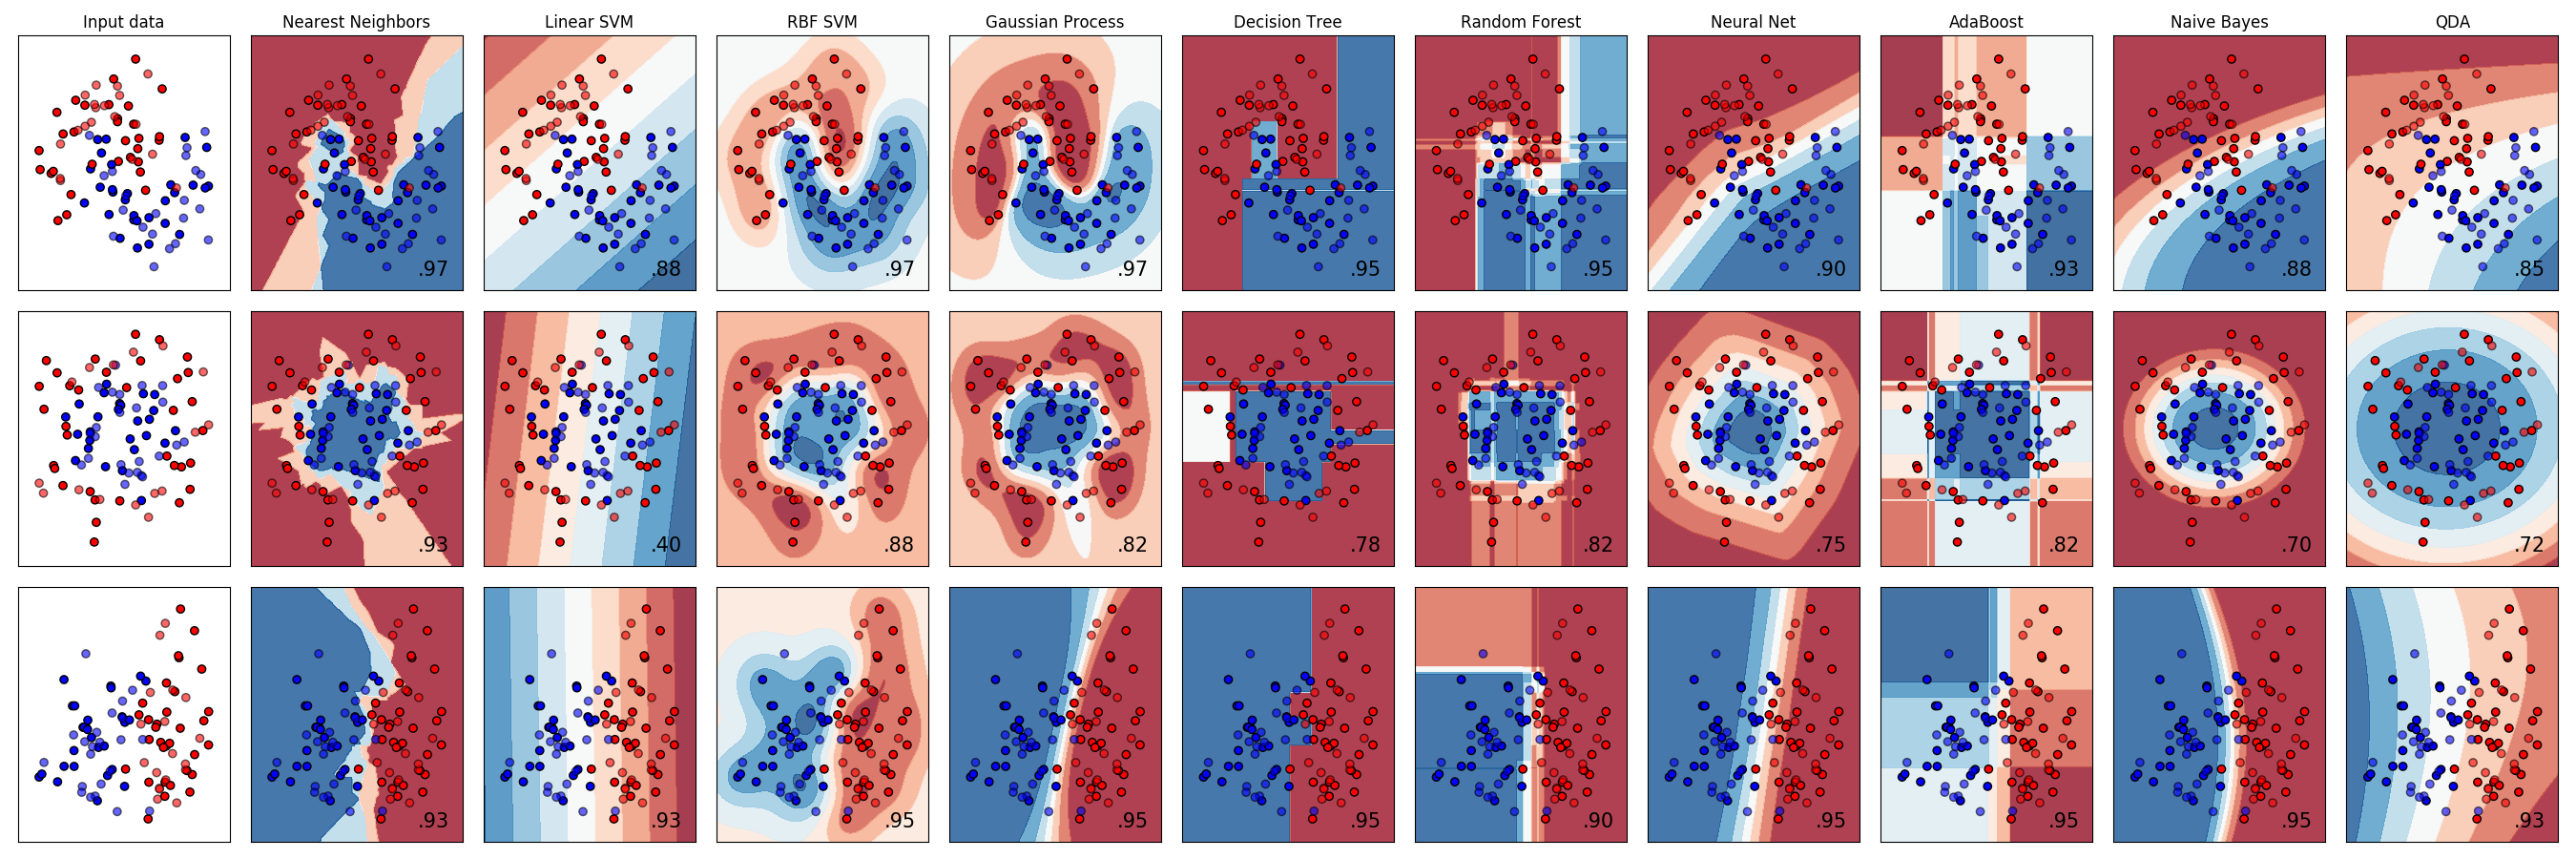
\includegraphics[width=\textwidth]{ml-decision-bounds.png}
\caption{Different of decision bounds as a result of different machine learning algorithms. Source: \protect\url{http://scikit-learn.org/stable/auto_examples/classification/plot_classifier_comparison.html} }\label{fig:ml-bounds}
 \end{figure}

\subsubsection{Gaussian Process}
The breakthrough results of deep convolutional neural networks in computer vision \cite{Krizhevsky2012} have sparked the interest of deploying similar systems for medical imaging diagnosis \cite{Greenspan2016}. However, one disadvantage of DNN is in its inability to quantify uncertainty and provide interpretable models. Model interpretability is a fundamental requirement for machine learning in medicine, and therefore there is renewed interest in bayesian-based models like Gaussian Process \cite{gal2016dropout}. DNN with an infinite number of hidden unit approximates GP \cite{neal1996priors}. 

Gaussian Process is defined as a collection of random variables, any finite number of which have a joint Gaussian distribution \cite{rasmussen2006gaussian}. 
It is a distribution that is defined by a mean function $m(x)$ and covariance function $k(x,x') $ where
\begin{equation}
	\begin{split}
		m(x) &= \mathbb{E}[f(x)], \\
		k(x,x') &= \mathbb{E}[(f(x)-m(x)(f(x')-m(x'))],
	\end{split}
\end{equation}
And the Gaussian Process is defined as
\begin{equation}
f(x) \sim GP(m(x), k(x, x')) 
\end{equation}

The covariance function is also termed called kernel function. The radial-basis function kernel or RBF kernel is widely used in machine learning tasks. The RBF kernel is also termed the square exponential, and is defined as

\begin{equation}
k(x, x') = exp\bigg( -\frac{1}{2}|x - x'|^2\bigg)
\end{equation} 

Another commonly used co-variance function is the Mat\'{e}rn kernel, which is used as an approximation for the RBF kernel in machine learning. It is defined, given a distance $r$ between two points, as:
\begin{equation}
k_{matern}(r) = \frac{2^{1-\nu}}{\Gamma(\nu)}\bigg(\frac{\sqrt{2\nu}r}{l}\bigg)^{\nu}K_{\nu}\bigg(\frac{\sqrt{2\nu}r}{l}\bigg)
\end{equation}
Where $K_\nu$ is a modified Bessel function \cite{rasmussen2006gaussian}. The Mat\'{e}rn kernel is equivalent to the RBF kernel when $\nu\rightarrow\infty$. In machine learning applications, $\nu$ commonly takes the value of $1.5$ or $2.5$ such that:
\begin{equation}
\begin{split}
k_{\nu=1.5}(d) &= \bigg(1+\frac{\sqrt{3}r}{l}\bigg)exp\bigg(-\frac{\sqrt{3}r}{l}\bigg), \\
k_{\nu=2.5}(d) &= \bigg(1+\frac{\sqrt{5}r}{l}+\frac{5r^2}{3l^2}\bigg)exp\bigg(-\frac{\sqrt{5}r}{l}\bigg), \\
\end{split}
\end{equation}
Where the function becomes once and twice differentiable respectively, and thereby having different degree of smoothness of approximation. 
 
\subsubsection{Training}
The process of fitting an ML model on labelled data to form predictions is called training. The objective of the training process is to obtain a model that can both correctly predict observed labels, and can generalize its predictions to new data that are not part of the training set. Depending on the model algorithm, there can be many training parameters that govern the model outcome. The tuning of these parameters is referred to as hyper-parameter tuning. It is possible for models trained with certain hyper-parameter combinations to result in model over-fitting, which is when a model is over-specialized in achieving the most accurate training label prediction, but perform poorly on unseen data. To properly evaluate model performance, a dataset is split into training/testing and validation sets, usually in 4:1 or 9:1 ratios, where model training is performed solely on the training set, and evaluation of model performance is on the validation set to assess the ability of the model to generalize.

There are instances when the number of available data is low, and each data point may have a substantial impact on model performance. In these cases, cross-validation is applied. The purpose is to divide the data into all possible combinations of training and validation splits, usually in the form of 5 fold to 10 fold. Then separate models are trained and evaluated on each combination, and their performance is averaged to form the final evaluation. This gives a reasonable approximate on the performance of the model when trained using all available data. Leave-one-out cross-validation is a special form where only one item is used for the validation split: given a dataset of N items, each split will consist of 1 and N-1 items, which result in N possible combinations. It is used when the available data are few. 
 
\subsection{Machine Learning, Neuroimaging, and Pain}

There is an extensive history of applying statistical methods to the field of neuroimaging, from the very onset of the field. Neuroimaging studies often attempt to correlate physiological and image-based measures with neuro-activities with specific experimental variables or conditions. Neuro-activities may be measured from EEG sensors, or as voxels in functional or structural MR images. Traditionally, data from each measured feature component was assumed to be independent. These components may be individual sensor readings or voxel-based measures. Correlative analysis were performed using general linear models, with post-hoc false-positive corrections. This type of univariate analysis does not have the ability to discover key relationships between feature components. Therefore univariate models cannot take into account spatial or temporally correlative dynamics. 

Increasing complexity in neuroimaging data has led to widespread applications of multi-variable machine learning methods in neuroimaging. Application of ML in pain neuroimaging became controversial when Tor Wager \cite{Wager2013} demonstrated a Lasso-PCA model that classified acute experimental pain with sensitivity and specificity of up to 90\% solely from fMRI imaging data. Additional studies showed consistently good performance of ML-based nociceptive pain discrimination. Discrimination of chronic pain from nociceptive pain proved to be more challenging, due to the high degree of similarity in activation patterns. The development of pain detection through brain imaging led to debates of the validity of presenting such methods as evidences in courtroom, where Davis et al argued against such actions \cite{Davis2012a}. While it is commonly accepted that pain evokes activity in the brain in multiple regions of the dynamic pain connectome, some studies suggest that the dorsal posterior-insula is heavily involved in chronic pain. Segerdale et al claimed that the dorsal posterior insula is a primary pain region \cite{Segerdahl2015a}, and this proposition ignited renewed debates surrounding regional specific brain centers for chronic pain \cite{Davis2015}.

Despite the controversies, interest in machine learning in medical imaging prognosis have sparked both public and private efforts across the globe. Classification studies using multi-modal data with features involving functional connectivity and structural connectivity in pain syndromes such as TN continue to improve. It is clear that machine learning is here to stay in pain neuroimaging research. 



